Hopefully with this worksheet we'll cover the set theory required for all of you to finish the homework good and proper.

 \begin{enumerate}
   \item It's important to realize the limitations of what kinds of sets we can define in our usual notation. The following example, independently discovered by Russel and Zermelo in the early 20th century illustrates that there cannot be a set of all sets. 

Suppose there was a universal set $U$, the set of all sets. Then $U$ contains itself (since $U$ is also a set).  Consider the subset of $U$ defined by
\[N = \{S \in U \mid S \not\in S\}.\] That is, $N$ contains all the sets $S$ which do not contain themselves.

\begin{enumerate}
    \item Show that $N$ is non-empty.
    \item Suppose $N \in N$. Deduce that $N \not\in N$. This is a contradiction, since formally we get the logical expression
    \[(N \in N) \land \lnot(N \in N) \equiv F.\]
    So then $N \not\in N$?
    \item But now suppose $N \not\in N$. Reason that $N \in N$.
\end{enumerate}
So the subset $N$ cannot exist. The conclusion is that the set $U$ is not well-defined (ie, does not exist).
   \item Fill in the table on page 2.
\begin{figure}[ht]
    \centering
    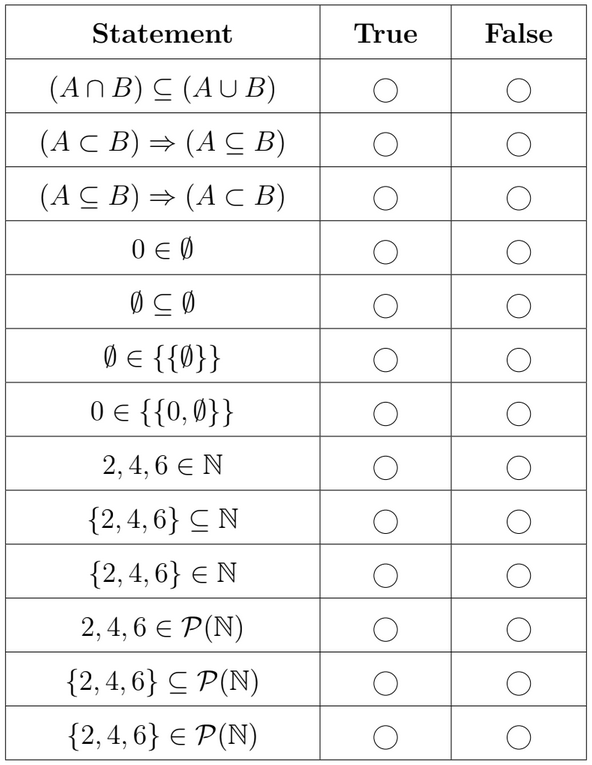
\includegraphics{Ch3/004.PNG}
    \label{fig:tf}
\end{figure}

Here are some definitions we will go over. $A$ and $B$ denote any sets.
\begin{itemize}
    \item $x \in A$ means an object $x$ is in the set $A$.
    \item $A \cup B = \{x \mid (x \in A) \lor (x \in B)\}$.
    \item $A \cap B = \{x \mid (x \in A) \land (x \in B)\}$.
    \item $A \subseteq B \iff ((x \in A) \implies (x \in B))$.
    \item $A \subset B \iff (A \neq B) \land (A \subseteq B)$.
    \item $\mathcal{P}(A) = \{U \mid U \subseteq A\}$. This is the \textbf{powerset} of $A$. 
    \item $|A|$ simply denotes the number of elements in the set $A$. For example, $|\{1, 2, 3\}| = 3$.
\end{itemize}
   \item This problem hopefully illustrates that the set cardinality operation is a ``depth $1$'' operation. All that matters when considering cardinality is the number of elements/objects in the first level of the set.

Determine the numbers for the sets below.
\begin{enumerate}
    \item $\vert \{3, 6, 9 \} \vert$
	\item $\vert \{ \{ 3\}, 6, 9 \} \vert$
	\item $\vert \{ \{3\}, 6, 9, \{ 9\} \} \vert$
	\item $\vert \{ \{ 3\}, 6, 9, \{ \{ 9 \}, 9\} \} \} \vert$
	\item $|\{\mathbb{R}\}|$
\end{enumerate}

   \item Just to get you used to the powerset operation. Compute $\mathcal{P}(\{a\})$, $\mathcal{P}(\{a, b\})$, and $\mathcal{P}(\{a, b, c\})$. Compute $\mathcal{P}(\mathcal{P}(\{a, b\}))$. 
   \item Last question, not really about set theory, but rather about quantifiers. Consider the propositional statement
   \[(\forall x \in \varnothing)[x = 5].\]
   Is this true? False? Discuss with your tablemates. After this, consider the proposition
   \[(\forall x \in \varnothing)[x \in A]\] where $A$ is any set. (Hopefully, from this we see that $\varnothing \subseteq A$ for all sets $A$!)
   % add more problem files here
 \end{enumerate}